        \documentclass{article}
\usepackage[margin=1in]{geometry}
\usepackage{hyperref}
\usepackage{amsmath,amsfonts,amssymb,amsthm,commath,dsfont}
\usepackage{enumitem}
\usepackage{framed}
\usepackage{xspace}
\usepackage{booktabs}
\usepackage{microtype}
\usepackage{float}
\usepackage[round]{natbib}
\usepackage{cleveref}
\usepackage[dvipsnames]{xcolor}
\usepackage{graphicx}
\usepackage{listings}
\usepackage[breakable]{tcolorbox}
\tcbset{breakable}
\usepackage{mathtools}
\usepackage{subcaption}
%\usepackage{symbols}

\usepackage{pifont}
\newcommand{\cmark}{\ding{51}}
\newcommand{\xmark}{\ding{55}}

\newcommand{\colbar}{\rule[-3mm]{.3mm}{1.5em}}
\newcommand{\rowbar}{\rule[.5ex]{1.5em}{.3mm}}
\DeclareMathOperator{\rank}{rank}

% following loops stolen from djhsu
\def\ddefloop#1{\ifx\ddefloop#1\else\ddef{#1}\expandafter\ddefloop\fi}
% \bbA, \bbB, ...
\def\ddef#1{\expandafter\def\csname bb#1\endcsname{\ensuremath{\mathbb{#1}}}}
\ddefloop ABCDEFGHIJKLMNOPQRSTUVWXYZ\ddefloop

% \cA, \cB, ...
\def\ddef#1{\expandafter\def\csname c#1\endcsname{\ensuremath{\mathcal{#1}}}}
\ddefloop ABCDEFGHIJKLMNOPQRSTUVWXYZ\ddefloop

% \vA, \vB, ..., \va, \vb, ...
\def\ddef#1{\expandafter\def\csname v#1\endcsname{\ensuremath{\boldsymbol{#1}}}}
\ddefloop ABCDEFGHIJKLMNOPQRSTUVWXYZabcdefghijklmnopqrstuvwxyz\ddefloop

% \valpha, \vbeta, ...,  \vGamma, \vDelta, ...,
\def\ddef#1{\expandafter\def\csname v#1\endcsname{\ensuremath{\boldsymbol{\csname #1\endcsname}}}}
\ddefloop {alpha}{beta}{gamma}{delta}{epsilon}{varepsilon}{zeta}{eta}{theta}{vartheta}{iota}{kappa}{lambda}{mu}{nu}{xi}{pi}{varpi}{rho}{varrho}{sigma}{varsigma}{tau}{upsilon}{phi}{varphi}{chi}{psi}{omega}{Gamma}{Delta}{Theta}{Lambda}{Xi}{Pi}{Sigma}{varSigma}{Upsilon}{Phi}{Psi}{Omega}{ell}\ddefloop

\newcommand\T{{\scriptscriptstyle\mathsf{T}}}
\def\diag{\textup{diag}}



\def\SPAN{\textup{span}}
\def\tu{\textup{u}}
\def\R{\mathbb{R}}
\def\E{\mathbb{E}}
\def\Z{\mathbb{Z}}
\def\be{\mathbf{e}}
\def\nf{\nabla f}
\def\veps{\varepsilon}
\def\cl{\textup{cl}}
\def\inte{\textup{int}}
\def\dom{\textup{dom}}
\def\Rad{\textup{Rad}}
\def\lsq{\ell_{\textup{sq}}}
\def\hcR{\widehat{\cR}}
\def\hcRl{\hcR_\ell}
\def\cRl{\cR_\ell}
\def\hcE{\widehat{\cE}}
\def\cEl{\cE_\ell}
\def\hcEl{\hcE_\ell}
\def\eps{\epsilon}
\def\1{\mathds{1}}
\newcommand{\red}[1]{{\color{red} #1}}
\newcommand{\blue}[1]{{\color{blue} #1}}
\def\srelu{\sigma_{\textup{r}}}
\def\vsrelu{\vec{\sigma_{\textup{r}}}}
\def\vol{\textup{vol}}
\def\hw{\textbf{[\texttt{hw2}]}\xspace}
\def\hwcode{\textbf{[\texttt{hw2code}]}\xspace}

\newcommand{\ip}[2]{\left\langle #1, #2 \right \rangle}
\newcommand{\mjt}[1]{{\color{blue}\emph\textbf{[M:}~#1~\textbf{]}}}
\newcommand{\sahand}[1]{{\color{green}\emph\textbf{[Sah:}~#1~\textbf{]}}}


\newtheorem{fact}{Fact}
\newtheorem{lemma}{Lemma}
\newtheorem{condition}{Condition}
\theoremstyle{definition}
\theoremstyle{remark}
\newtheorem{remark}{Remark}
\newtheorem{example}{Example}

\newenvironment{Q}
{%
	\clearpage
	\item
}
{%
	\phantom{s} %lol doesn't work
	\bigskip
	\textbf{Solution.}
}

\title{CS 446 / ECE 449 --- Homework 2}
\author{\emph{acard6}}
\date{}

\begin{document}
	\maketitle
	
	\noindent\textbf{Instructions.}
	\begin{itemize}
		\item
		Homework is due \textbf{\color{red}Tuesday, Feb. 21, at noon CDT}; no late homework accepted.
		
		\item
		Everyone must submit individually at gradescope under \texttt{hw2} and \texttt{hw2code}.
		
		\item
		The ``written'' submission at \texttt{hw2} \textbf{must be typed}, and submitted in
		any format gradescope accepts (to be safe, submit a PDF).  You may use \LaTeX, markdown,
		google docs, MS word, whatever you like; but it must be typed!
		
		\item
		When submitting at \texttt{hw2}, gradescope will ask you to mark out boxes
		around each of your answers; please do this precisely!
		
		\item
		Please make sure your NetID is clear and large on the first page of the homework.
		
		\item
		Your solution \textbf{must} be written in your own words.
		Please see the course webpage for full academic integrity information.
		Briefly, you may have high-level discussions with at most 3 classmates,
		whose NetIDs you should place on the first page of your solutions,
		and you should cite any external reference you use; despite all this,
		your solution must be written in your own words.
		
		\item
		We reserve the right to reduce the auto-graded score for
		\texttt{hw2code} if we detect funny business (e.g., your solution
		lacks any algorithm and hard-codes answers you obtained from
		someone else, or simply via trial-and-error with the autograder).
		
		\item
		When submitting to \texttt{hw2code}, only upload \texttt{hw2\_ResNet.py}. Additional files will be ignored.
		
		\item
		Gradescope coding questions are marked by ``\texttt{[code]}.''
		
	\end{itemize}
	
	
	\begin{enumerate}[font={\Large\bfseries}]
        \input{EM.tex} 
		\begin{itemize}
			\item[\textit{Answer A.i)}] A given D $~$ bernoulli distribution is $P(D|\theta) =\theta^x(1-\theta)^{1-x}$ therefore the likelihood P becomes 
			$$P(x|q) = \Pi_{d=1}^D q_d^{x_d}(1-q_d)^{1-x_d}$$\\
			
			\item[\textit{Answer A.ii)}] {$P(x^i |\pi,p) = \sum_{k=1}^K \pi_k Bern(x^i | p^k) = \sum_{k=1}^K \pi_k P(x^i|p^k) =\\
			 \sum_{k=1}^K \pi_k \Pi_{d=1}^D (p_{d}^{k})^{x_{d}^{i}}(1-p_{d}^{k})^{1-x_{d}^{i}}$}\\
		
			\item[\textit{Answer A.iii)}] $P(\mathcal{D}|\pi,p) = 
			\Pi_{i=1}^n(P(x^i|\pi,p)) = 
			\Pi_{i=1}^n(\sum_{k=1}^K\pi_k P(x^i|\pi,p)) \rightarrow \\
			log(P(\mathcal{D}|\pi,p)) = 
			\sum_{i=1}^n \log(P(x^i|p,\pi)) = 
			\\\sum_{i=1}^n(\sum_{k=1}^K\pi_k P(x^i|\pi,p)) = 
			\sum_{i=1}^n(\log(\sum_{k=1}^K\pi_k (\sum_{d=1}^D (p_{d}^{k})^{x_{d}^{i}}(1-p_{d}^{k})^{1-x_{d}^{i}})))$\\

			\item[\textit{Answer B.i)}] $P(z^i| \pi) = \Pi_{k=1}^K \pi_k^{z_k^i}$\\

			\item[\textit{Answer B.ii)}] $P(x^i|z^i,p,\pi) = \Pi_{k=1}^K \pi_k^{z_k^i} = \Pi_{k=1}^K (P(x^i|p^k)^{z_k^i})$\\
			
			\item[\textit{Answer B.iii)}] $P(Z,\mathcal{D}|pi,p) = \Pi^n_{i=1} P(x^i,z^i| p, \pi) = \Pi^n_{i=1} P(x^i|z^i, p, \pi)P(z^i|\pi) =\\ 
			\Pi^n_{i=1} \Pi^K_{k=1} \pi_k^{z_k^i} (P(x^i|p^k))^{z_k^i}$\\

			\item[\textit{Answer B.iv)}] $\eta(z_k^i) = 
			\mathbb{E} [z_{k}^{(i)}| x^{(i)},\pi,p] = 
			P(z_k^i=1|x^i,p,\pi) = 
			\frac{P(z^i_k=1|\pi,p)P(x^i|z^i_k=1,\pi,p)}{\sum_{j} P(z^i_{j}=1)P(x^i|z^i_{j},\pi,p)} = \\
			\frac{\pi_kP(x^i|p^k)}{\sum_j \pi_jP(x^i|p^j)} = 
			\frac{\pi_k \Pi_{d=1}^D (p_{d}^{k})^{x_{d}^{i}}(1-p_{d}^{k})^{1-x_{d}^{i}}}{\sum_j \pi_j \Pi_{d=1}^D (p_{d}^{j})^{x_{d}^{i}}(1-p_{d}^{j})^{1-x_{d}^{i}}}$\\

			\item[\textit{Answer B.v)}] $log P(Z, \mathcal{D}|\tilde{p},\tilde{\pi}) = 
			[\sum_{i=1}^{n} \sum_{k=1}^{K} z_k^i log(P(x^i|p^i))] +[\sum_{k=1}^{K}z_k^i \log(pi_k)] =\\ 
			\sum_{i=1}^{n} \sum_{k=1}^{K} z_k^i [log(P(x^i|p^i)) + \log(\pi_k)] = \\
			\sum_{i=1}^{n} \sum_{k=1}^{K} z_k^i [\log(\pi_k) + \sum_{d=1}^{D} (x^i_d)\log(p_d^k)+(1-x^i_d) \log(1-p_d^k)]$\\
			taking the expectation of the previous equation we note $\mathbb{E}[z_k^i]=\eta(z_k^i)$ and leaving eveerything else to be the maximized parameters we arrive at:
			$$\mathbb{E} [log P(Z, \mathcal{D}|\tilde{p}, \tilde{\pi}) | \mathcal{D}, p, \pi] = 
			\sum_{i=1}^{n} \sum_{k=1}^{K} \eta(z_k^i) [\log(\tilde{\pi}_k) + \sum_{d=1}^{D} (x^i_d)\log(\tilde{p}_d^k)+(1-x^i_d) \log(1-\tilde{p}_d^k)]$$\\

			\item[\textit{Answer C.i)}] $\frac{d}{dp^{(k)}} = \mathbb{E} [log P(Z, \mathcal{D}|p,\pi)] = \sum_{i=1}^{n} \eta(z_k^i)[\frac{x^i}{p^k}+\frac{1-x^i}{1-p^k}]=0 \rightarrow\\
			\sum_{i=1}^{n} \eta(z^i_k)[x^i(1-p^k)+p^k(1-x^i)] = 0, \rightarrow 
			\sum_{i=1}^{n} \eta(z^i_k)[x^i - p^k] = 0, \rightarrow\\
			\sum_{i=1}^{n} \eta(z^i_k) x^i = \sum_{i-1}^{n} \eta(z_k^i) p^k \rightarrow \tilde{p}^k = \frac{\sum_{i=1}^{n} x^i \eta(z_k^i)}{\sum_{i=1}^{n} \eta(z_k^i)} \rightarrow
			\tilde{p}^{(k)} = \frac{\sum_{i=1}^{n} x^i \eta(z_k^i)}{N_k}$\\

			\item[\textit{AnswerC.ii)}] $\frac{d}{d\pi_k}\mathbb{E}[logP(Z, \mathcal{D}|p,\pi)] = 
			\frac{d}{d\pi_k} \sum_{i} \sum_{k} \eta(z_k^i) \log(\pi_k) + \lambda (\sum_k \pi_k) =\\
			\sum_{i=1}^n \frac{\eta(z_k^i)}{\pi_k} + \lambda \rightarrow
			\pi_{k} = \frac{\sum_{i=1}^n \eta(z_k^i)}{\lambda} = \frac{N_k}{\lambda}$\\
			solving for the lagrangian multiplier we take the derivative w.r.t $\lambda$, we get:\\
			$\frac{d}{d\lambda} \sum_i \sum_k \eta(z_k^i)\log (N_k-\lambda) + (\sum_k N_k - \lambda) \rightarrow 
			\frac{1}{\lambda} \sum_i \sum_k \eta(z_k^i) - 1 = 0 \rightarrow\\
			\lambda = \sum_{k=1}^K N_k \rightarrow \tilde{\pi}_k = \frac{N_k}{\sum_{\hat{k}} N_{\hat{k}}}$

		\end{itemize}
		
        \begin{Q}
\textbf{\Large Deep Net}\\ 

We want to train a simple deep net $f(w_3, w_2, w_1, x) = w_3\sigma_2(\underbrace{w_2\sigma_1(\underbrace{w_1x}_{x_1})}_{x_2})$ where $w_1, w_2, w_3, x\in\mathbb{R}$ are real valued and $\sigma_1(u) = \sigma_2(u) = \frac{1}{1+\exp(-u)}$ is the sigmoid function.

\begin{enumerate}
% Subproblem description
\item{Draw the computation graph that is specified by the function $f$.
}

 % Subproblem description
\item{Compute $\frac{\partial \sigma_1}{\partial u}$ and provide the answer (1) using only $u$, the $\exp$-function and the square function, and (2) using only $\sigma_1(u)$.
}

% Subproblem description
\item{Describe briefly what is meant by a `forward pass' and a `backward pass'?
}
% Subproblem description
\item{Compute $\frac{\partial f}{\partial w_3}$. Which result should we retain from the forward pass in order to make computation of this derivative easy?

}
 
 % Subproblem description
\item{Compute $\frac{\partial f}{\partial w_2}$. Make use of the second option obtained in part (b). Which results should we retain from the forward pass in order to make computation of this derivative easy?
}

% Subproblem description
\item{Compute $\frac{\partial f}{\partial w_1}$. Make use of the second option obtained in part (b). Which results should we retain from the forward pass in order to make computation of this derivative easy? In what order should we compute the derivatives $\frac{\partial f}{\partial w_3}$, $\frac{\partial f}{\partial w_2}$ and $\frac{\partial f}{\partial w_1}$ in order to obtain the result as early as possible and in order to reuse as many results as possible. How is this order related to the forward pass?
}

% Subproblem description
\item{We now want to train a convolutional neural net for 10-class classification of MNIST images which are of size $28\times 28$. As a first layer we use 20 2d convolutions each with a filter size of $5 \times 5$, a stride of 1 and a padding of 0. What is the output dimension after this layer? Subsequently we apply max-pooling with a size of $2\times 2$. What is the output dimension after this layer?
}


% Subproblem description
\item{After having applied the  two layers (convolution + pooling) designed in part (g)  we want to use  a second convolution + max-pooling operation. The max-pooling operation has a filter size of $2\times 2$. The desired output should have 50 channels and should be of size $4 \times 4$. What is the filter size, the stride, and the channel dimension of the second convolution operation, assuming that padding is 0?
}


\end{enumerate}

\end{Q}
		\begin{itemize}
			\item[\textit{Answer A.)}] 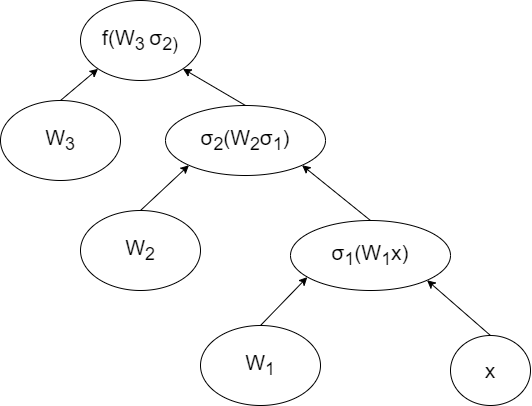
\includegraphics[scale=0.2]{deepNetDrawing.png}\\
			\textbf{figure 1:} the drawing for Q2 part a\\

			\item[\textit{Answer B.)}] $\frac{\delta \sigma_1}{\delta u} =
			\frac{\delta}{\delta u} \frac{1}{1+e^{-x}} = 
			\frac{e^{-u}}{(1+e^{-u})^2} = 
			\sigma_1(1 - \sigma_1)$\\

			\item[\textit{Answer C.)}] \textbf{Forward pass} is when you propogate your inputs through the deep net going through each layer and
			measure the prediction made as an error.\\
			\textbf{Backward pass} we start by measuring the error of a prediction to the output from a hidden layer until reaching the input and
			computing an input that would get the output that was chosen.

			\item[\textit{Answer D.)}] $\frac{\delta f}{\delta w_3} = 
			\frac{\delta}{\delta w_3} w_3 \sigma_2 (w_2 \sigma_1 (w_1 x)) = \sigma_2 (w_2 \sigma_1 (w_1 x))$\\
			We should retain the output of the second layer from the forward pass since the derivative w.r.t $w_3$ is just that value and retaining
			it will make deriving for back propogation easier since we have retained that value already
			
			\item[\textit{Answer E.)}] $\frac{\delta f}{\delta w_2} = 
			\frac{\delta f}{\delta \sigma_2(x_2)} \frac{\delta \sigma_2(x_2)}{\delta x_2} \frac{\delta x_2}{\delta w_2} \rightarrow
			\frac{\delta f}{\delta \sigma_2(x_2)} = w_3, 
			\frac{\delta \sigma_2(x_2)}{\delta x_2} = \sigma_2 (1-\sigma_2), 
			\text{ and } \frac{\delta x_2}{\delta w_2} = \sigma_1(x_1)$
			$$\frac{\delta f}{\delta w_2} = w_3 \sigma_2(x_2) (1-\sigma_2(x_2)) \sigma_1(x_1)$$
			we would save the output of the function and the output of the second layer and 1 minus the second layer and the output of the first layer,
			since we would then multiply those 4 values for back propogation
			
			\item[\textit{Answer F.)}] repeating the same process as E for $w_1$ instead leads to\\ 
			$\frac{\delta f}{\delta w_2} = 
			\frac{\delta f}{\delta \sigma_2} \frac{\delta \sigma_2}{\delta x_2} \frac{\delta x_2}{\delta \sigma_1} \frac{\delta \sigma_1}{\delta x_1} \frac{\delta x_1}{\delta w_2} \rightarrow 
			\frac{\delta x_2}{\delta \sigma_1} = w_2, 
			\frac{\delta \sigma_1}{\delta x_1} = \sigma_1 (1-\sigma_1), 
			\frac{\delta x_1}{\delta w_2} = x$
			$$\frac{\delta f}{\delta w_2} = w_3 \sigma_2(1-\sigma_2) w_2 \sigma_1(1-\sigma_1) x$$
			we would need to retain the final output, the output to the second layer, the input to the second layer, the output to the first layer
			and the input of out finction to be able to do back propogation. We should compute the derivatives in reverse order meaning we take
			the last derivative (the last layer) first and then work backward towards the first derivative (first layer) since we need to know the
			last derivative to be able to do all the derivatives since the previous layer just involves tacking on a bit of math the layer infront of it.
			This order relates to the opposite of forward pass.

			\item[\textit{Answer G.)}] the dimensions of convolution output are calculated as $[(I - F + 2*S)/2]+1$, where I is the input size, 
			F is the filter size, P is the padding, and S is the stride we get $Dim = [(28 - 5 + 2 * 0) / 1] + 1 = 24$. So the dimensions is 24 x 24 x 20\\
			After Applying a max-pooling with size 2x2, we assume S=2 and divide the dimensions by S to get $(\frac{24}{2},\frac{24}{2},20) $= 12 x 12 x 20. 

			\item[\textit{Answer H.)}] to reduce to a size of 4, the function $[(I-F+2P/S)]+1=4$, assuming I=12 and P=0 , we get F=12-3S.
			If we want 50 channels we need to solve $(I_C - F_C + 2P)/S + 1 = 50 \rightarrow (12 - (12-4S)/S) + 1 = 50 \rightarrow S=\frac{1}{12}$
			, after solving this equation for F knowing S=1/12 we get F=11, so the convolution layer becomes 2x2x20
		\end{itemize}

        \begin{Q}
    \textbf{\Large ResNet.}
    
    In this problem, you will implement a simplified ResNet. You do not need to change arguments which are not mentioned here (but you of course could try and see what happens).
    \begin{enumerate}
        \item \texttt{[code]} Implement a class \texttt{Block}, which is a building block of ResNet. It is described in Figure 2 of \citet{resnet}, but also as follows.

        The input to \texttt{Block} is of shape $(N,C,H,W)$, where $N$ denotes the batch size, $C$ denotes the number of channels, and $H$ and $W$ are the height and width of each channel. For each data example $\vx$ with shape $(C,H,W)$, the output of \texttt{block} is
        \begin{align*}%\label{eq:block}
            \texttt{Block}(\vx)=\sigma_r\del{\vx+f(\vx)},
        \end{align*}
        where $\sigma_r$ denotes the ReLU activation, and $f(\vx)$ also has shape $(C,H,W)$ and thus can be added to $\vx$. In detail, $f$ contains the following layers.
        \begin{enumerate}
            \item A \texttt{Conv2d} with $C$ input channels, $C$ output channels, kernel size 3, stride 1, padding 1, and no bias term.
            \item A \texttt{BatchNorm2d} with $C$ features.
            \item A ReLU layer.
            \item Another \texttt{Conv2d} with the same arguments as i above.
            \item Another \texttt{BatchNorm2d} with $C$ features.
        \end{enumerate}
        Because $3\times3$ kernels and padding 1 are used, the convolutional layers do not change the shape of each channel. Moreover, the number of channels are also kept unchanged. Therefore $f(\vx)$ does have the same shape as $\vx$.

        Additional instructions are given in doscstrings in \texttt{hw2\_ResNet.py}.
        
        \textbf{Library routines:} \texttt{torch.nn.Conv2d and torch.nn.BatchNorm2d.}
        
        \textbf{Remark:} Use \texttt{bias=False} for the \texttt{Conv2d} layers.

        \item \texttt{[code]}  Implement a (shallow) \texttt{ResNet} consists of the following parts:
        \begin{enumerate}
            \item A \texttt{Conv2d} with 1 input channel, $C$ output channels, kernel size 3, stride 2, padding 1, and no bias term.
            \item A \texttt{BatchNorm2d} with $C$ features.
            \item A ReLU layer.
            \item A \texttt{MaxPool2d} with kernel size 2.
            \item A \texttt{Block} with $C$ channels.
            \item An \texttt{AdaptiveAvgPool2d} which for each channel takes the average of all elements.
            \item A \texttt{Linear} with $C$ inputs and 10 outputs.
        \end{enumerate}
        Additional instructions are given in doscstrings in \texttt{hw2\_ResNet.py}.
        
        \textbf{Library routines:} \texttt{torch.nn.Conv2d, torch.nn.BatchNorm2d, torch.nn.MaxPool2D,}
        
        \texttt{torch.nn.AdaptiveAvgPool2d and torch.nn.Linear.}
        
        \textbf{Remark:} Use \texttt{bias=False} for the \texttt{Conv2d} layer.
        
        
        \item  Train your \texttt{ResNet} implemented in (b) with different choices $C\in\{1,2,4\}$ on digits data and draw the training error vs the test error curves. To make your life easier, we provide you with the training script \texttt{utils\_train\_script.py} to load the digits data and train your ResNet with different choices for $C$. Therefore, you only need to plot the training and testing errors. Train your algorithms for 4000 epochs using SGD with mini batch size 128 and step size 0.1. See the docstrings in \texttt{hw2\_ResNet.py} for more details.  Include the resulting plot in your written handin. 
        
          For full credit, in addition to including the six train and test curves,
          include at least one complete sentence describing how the train and test error (and in particular their gap) change with $C$, which itself corresponds to a notion of model complexity as discussed in lecture.
        
         \textbf{Library routines:} \texttt{torch.nn.CrossEntropyLoss, torch.autograd.backward, torch.no\_grad, torch.optim.Optimizer.zero\_grad, torch.autograd.grad, torch.nn.Module.parameters.}
         
     \item Train your \texttt{ResNet} implemented in (b) with $C=64$ on digits data and draw the training error vs the test error curve. You may use the same training script provided for the previous question to train your ResNet with $C=64$. Train your algorithms for 4000 epochs using SGD with mini batch size 128 and step size 0.1. See the docstrings in \texttt{hw2\_ResNet.py} for more details. Include the resulting plot in your written handin. 
                
         For full credit, additionally include at least one complete sentence comparing the train and test error with those in part (c).
         
         \textbf{Library routines:} \texttt{torch.nn.CrossEntropyLoss, torch.autograd.backward, torch.no\_grad, torch.optim.Optimizer.zero\_grad, torch.autograd.grad, torch.nn.Module.parameters.}
    \end{enumerate}
\end{Q}
 
        	\begin{itemize}
        	\item[\textit{Answer C)}].\\
			\centering
        		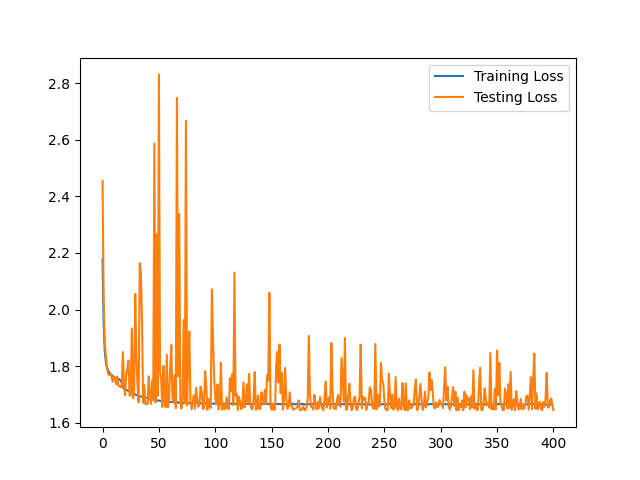
\includegraphics[scale=0.6]{loss_c_1.png}\\
			\textbf{figure 2:} the plot if training and testing loss for C=1\\
        	\end{itemize}
		
	\end{enumerate}

\newpage

\bibliography{shortbib}
\bibliographystyle{plainnat}

\end{document}
